\chapter{Система планирования производства}

\section{Архитектура системы планирования}

\begin{figure}[H]
    \center{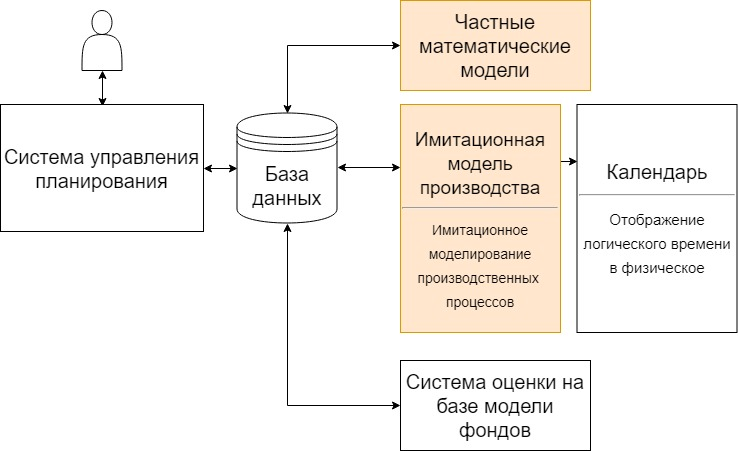
\includegraphics[width=1\linewidth]{fig/arh1.jpg}}
    \caption{Архитектура ПО}
    \label{ris:arh1}
\end{figure}

На рисунке \ref{ris:arh1} представлена архитектуры программного обеспечения. Данная архитектура содержит следующие элементы:

\begin{itemize}
    \item пользовательский интерфейс для взаимодействия с системой, который также позволяет получать информацию о работе системы в виде диаграмм, или графиков; 
    \item система управления планирования взаимодействует со всеми элементами системы и является главным распорядителем задач;
    \item база данных хранит всю информацию о производстве и результаты планирования; 
    \item основная задача имитационной модели заключается в построении расписания, в котором указаны все операции, время их начала и окончания, время начала и окончания участия производственных ресурсов в выполнения операций.
    \item календарь обрабатывает абсолютные значения, используемые при планировании, и привязывает их к конкретным датам;
    \item частные оптимизационные модели работают с уже сформировавшимся планом, который получен в результате имитационного моделирования. К данному плану применяются алгоритмы оптимизации, зависящие от конкретных целей. Таким целями могут быть: задачи упорядочивания, задачи согласования, задачи распределения, задачи с суммарными критериями оптимизации, задачи с минимаксимальными критериями оптимизации[1, 2].
    \item модель оценки фондов работает с производственными мощностями и дают поверхностную оценку осуществимости заданной цеховой последовательности выпуска;
\end{itemize}

\section{Организация системы имитацонного моделирования}

\subsection{Формализация предметной области}

Для того, чтобы разрабатывать алгоритмы планирования в первую очередь необходимо формализовать предметную область. В данном случае формализуется сборочный цех со значимыми внутренними особенностями.

Как правило на любом предприятии имеется специальный документ – технологическая карта, детально описывающая весь перечень операций по достижению которых воспроизводится единица продукции. Технологическая карта хранит информацию о зависимостях между операциями, привязках ресурсов к операциям, трудоёмкостях операций, периодичность операций, результат каждой операции. 

Далее важно учесть ресурсы предприятия. В рамках сборочного производства такими ресурсами могут быть: персонал, оборудование, организация конвейерной производственной линии.

Последним пунктом для построения модели производства является производственный план. То есть перечень продукции в составе заказа и срок реализации данного заказа. На рисунке \ref{ris:Prod1} представлен пример взаимодействия перечисленных выше моделей. 

\begin{figure}[H]
    \center{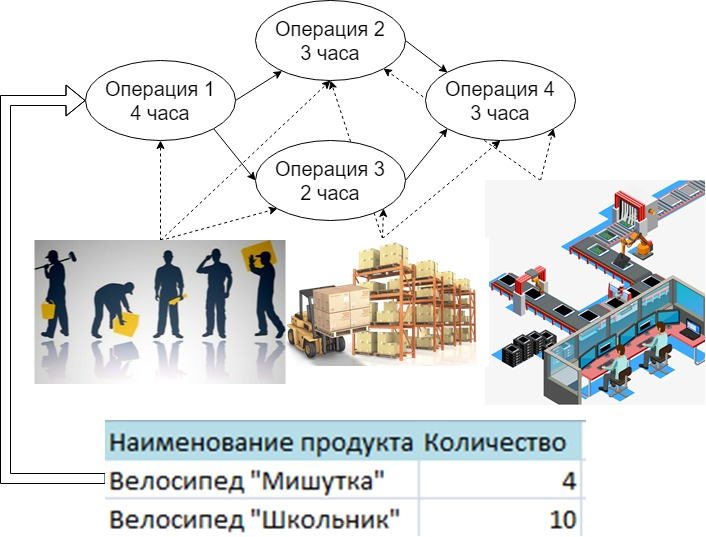
\includegraphics[width=1\linewidth]{fig/Prod1.jpg}}
    \caption{Модель производства}
    \label{ris:Prod1}
\end{figure}

\subsection{Математическое моделирование производственных процессов}

Для формализации процесса планирования в работе используются системы неравенств. Пример системы неравенств представлена на рисунке \ref{ris:sys1}. Система неравенств состоит из двух частей: статическую и динамическую. Статическая по своей сути копирует последовательность операций, описываемых в технологической карте. Динамическая накладывает дополнительные ограничения на систему неравенств, которая складывается из ресурсных зависимостей. Ресурсными зависимостями являются связи между операциями и фондом предприятия[3].

\begin{figure}[H]
    \center{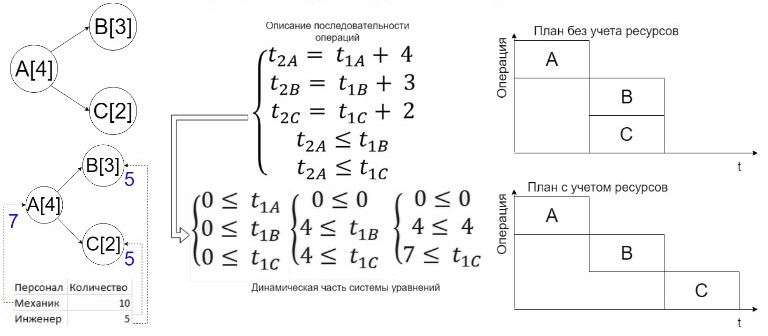
\includegraphics[width=1\linewidth]{fig/Screenshot_3.jpg}}
    \caption{Система неравенств}
    \label{ris:sys1}
\end{figure}

Таким образом планирование делится на шаги, каждый раз при этом формируются новые ограничения вводимые ресурсами.

По результатам анализа работы \cite{Jahangirian}, была составлена градация подходов к имитационному планированию представленная на рисунке \ref{ris:IM_detalApp}. 

Решение задачи планирования аналитическим подходом возможна, при этом основная проблема заключается в сложности описания всех зависимостей, что делает данный подход сложным в исполнении.

Второй крайностью решения задач имитационного моделирования является объектно-ориентированный подход. Одним из примеров реализации данной идеи является Siemens Plant Simulation.


\begin{figure}[H]
    \center{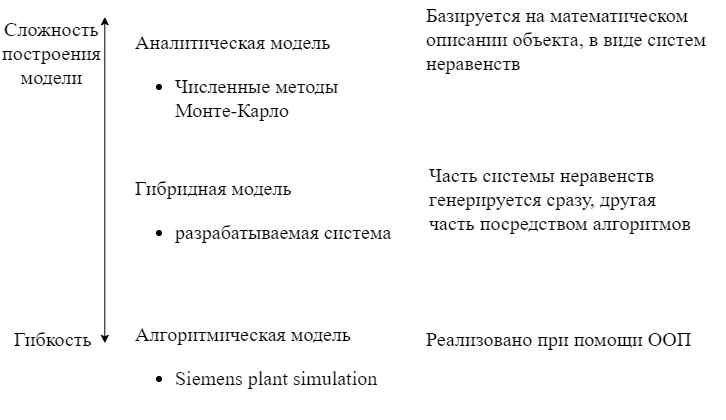
\includegraphics[width=1\linewidth]{fig/IM_detalApp.png}}
    \caption{Градация подходов к имитационному моделированию}
    \label{ris:IM_detalApp}
\end{figure}


\section{Частные оптимизационные модели}

В данном разделе приведено описание частных оптимизационных моделей. Необходимость применения данных моделей возникла, с появлением задач оптимизации на специфичных производствах. Данная специфика характеризуется уникальным для каждого предприятия структуры, где стандартные методы оптимизации будут не эффективны, либо не будут давать результата.

На текущий момент представлена одна частная оптимизационная модель, задача которой оптимизация сборочных производств. Сборочные производства характеризуются сборочными линиями, где на разных этапах установлены рабочие станции. Рабочий процесс на таком производстве выглядит следующим образом, загатовка перемещается от станции к станции, при этом на каждой станции ведется своя независимая работа.

Целью оптимизции является равномерная загрузка всех станций на линии, чтобы избежать простоя производства. Для достижения данной цели были созданы модели необходимые для описания сборочного производства. Такими моделями являются ресурс рабочих, а также модель конвейера. Также разработаны методы оптимизации описанные в главе \ref{ALBP}.

\section{Выбор технологии реализации}

Планированию как вычислительному процессу необходимо большое количество вычислительных ресурсов и их грамотное использование. Это связано с тем фактом, что при планировании перебираются множество возможных вариантов и выбирается только один - лучший (в данном случае имеются в виду алгоритмы оптимального поиска). Когда речь идет о возможности распараллеливания вычислительных ресурсов, требуется технология предоставляющая данную возможность. На данный момент практически все языки программирования имеют функцию распараллеливания, но языки, где это реализовано удобно и без изъянов, немного.  Для построения ядра моделирования был выбран многопоточный, компилируемый язык программирования - golang.

Язык программирпования golang предоставляет следующие возможности:

\begin{enumerate}
    \item Скорость обучения. Часто бывает, что разработчики имеют разный уровень подготовки, поэтому необходим язык который позволяет уменьшить затраты на изучения синтаксиса и как можно быстрее сосредоточиться на разработке. 
    \item Производительность. Golang компилируемый язык. 
    \item Эффективность и возможность многопоточности. В Go есть горутины. Горутинами называют функцию, которая выполняется с другими гортинами в едином адресном пространстве. Основными преимуществами горутин являются: низкое потребление памяти(4,5 кб), минимум накладных ресурсов на организацию, а также простота использования.
    \item Встроенный сборщик мусора.
\end{enumerate}

Язык программирования golang вобрал преимущества низкоуровневых языков(сразу компилируется в двоичный код), а также высокоуровневых(имеет сборщик мусора для распределения и удаление объектов). Так как главный акцент, при выборе языка программирования, делался на производительность и поддержку многопоточности, golang является лучшим вариантом для создания ядра моделирования производственного плана. 

Данный акцент на быстроте и многопточности был сделан не случайно. Как будет видно далее в вопросах поиска оптимальных решений данные особенности golang будут очень востребованы.